\documentclass[12pt]{article}

\usepackage[utf8]{inputenc}
\usepackage[T2A]{fontenc}
\usepackage[ukrainian]{babel}
\usepackage{geometry}
\geometry{a4paper, margin=2cm}

\usepackage{xcolor}
\usepackage[most]{tcolorbox}
\usepackage{graphicx}
\usepackage{amsmath, amsthm, amssymb}
\usepackage{caption}
\captionsetup{labelsep=period}

\usepackage{fancyhdr}
\pagestyle{fancy}
\fancyhf{}
\setlength{\headheight}{15pt}
\fancyfoot[C]{\thepage}

\newtheorem{theorem}{Теорема}

\begin{document}

\begin{center}
    {\LARGE \textbf{Трикутник та його основні властивості}}
\end{center}

\section{Короткі теоретичні відомості}

\begin{tcolorbox}[colback=blue!10!white, colframe=blue!80!black, title=Визначення]
Трикутник --- це геометрична фігура, що складається з трьох точок, які не лежать на одній прямій, і трьох відрізків, що сполучають ці точки.
\end{tcolorbox}

Позначення:
\begin{itemize}
\item $a, b, c$ --- сторони трикутника;
\item $\alpha, \beta, \gamma$ --- кути;
\item $p = \frac{a+b+c}{2}$ --- півпериметр;
\item $S$ --- площа.
\end{itemize}

На рисунку \ref{fig:triangle1} зображено трикутник з основними позначеннями.

\begin{figure}[h]
    \centering
    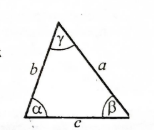
\includegraphics[width=0.4\textwidth]{triangle1.png}
    \caption{Трикутник $ABC$ з позначеннями}
    \label{fig:triangle1}
\end{figure}

\section{Основні лінії в трикутнику}

\begin{tcolorbox}[colback=blue!10!white, colframe=blue!80!black, title=Визначення]
Бісектриса трикутника --- це відрізок, який ділить кут навпіл.
\end{tcolorbox}

Як показано на рисунку \ref{fig:triangle2}, бісектриса ділить протилежну сторону пропорційно прилеглим сторонам.

\begin{figure}[h]
    \centering
    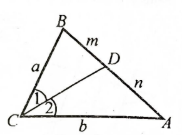
\includegraphics[width=0.4\textwidth]{triangle2.png}
    \caption{Бісектриса трикутника}
    \label{fig:triangle2}
\end{figure}

\section{Основні співвідношення}

\begin{enumerate}
    \item $\alpha + \beta + \gamma = 180^\circ$
    \item $b + c > a$
    \item \[
    \frac{a}{\sin \alpha} = \frac{b}{\sin \beta} = \frac{c}{\sin \gamma}
    \]
\end{enumerate}

\section{Теорема і доведення}

\begin{theorem}
Сума кутів трикутника дорівнює $180^\circ$.
\end{theorem}

\begin{proof}
Проведемо через вершину пряму, паралельну протилежній стороні.
Отримуємо розгорнутий кут, що дорівнює $180^\circ$.
\end{proof}

\section{Прямокутний трикутник}

На рисунку \ref{fig:triangle3} показано прямокутний трикутник.

\begin{figure}[h]
    \centering
    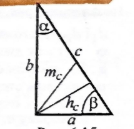
\includegraphics[width=0.4\textwidth]{triangle3.png}
    \caption{Прямокутний трикутник}
    \label{fig:triangle3}
\end{figure}

Теорема Піфагора:
\[
a^2 + b^2 = c^2
\]

\section{Приклад}

Нехай $a=3$, $b=4$.

\[
c = 5
\]

\[
S = \frac{1}{2}ab = 6
\]

\section{Висновок}

Було розглянуто трикутник, його властивості, теореми та наведено ілюстрації.

\end{document}